\documentclass{article}[12pt]
\usepackage{color}
\usepackage[normalem]{ulem}
\usepackage{times}
\usepackage{fullpage}
\usepackage{amsmath}
\usepackage{amssymb}
\usepackage{tikz}
\def \R {\mathbb R}
\def \imp {\Longrightarrow}
\def \eps {\varepsilon}
\def \Inf {{\sf Inf}}
\newenvironment{proof}{{\bf Proof.  }}{\hfill$\Box$}
\newtheorem{theorem}{Theorem}[section]
\newtheorem{definition}{Definition}[section]
\newtheorem{corollary}{Corollary}[section]
\newtheorem{lemma}{Lemma}[section]
\newtheorem{claim}{Claim}[section]
\setlength {\parskip}{2pt}
\setlength{\parindent}{0pt}

\newcommand{\headings}[4]{\noindent {\bf Assignment 6 CME241} \hfill {{\bf Author:} Nicolas Sanchez} \\
{} \hfill {{\bf Due Date:} #2} \\

\rule[0.1in]{\textwidth}{0.025in}
}

\newcommand{\klnote}[1]{{\color{red} #1}}
\newcommand{\klsout}[1]{{\color{red} \sout{#1}}}

\begin{document}

\headings{\#1}{Tuesday, October 8, 10:30am}\section{} 



\section{Merton's Continuous Time Formulation}
We have the following setup:
\begin{align*}
dW_t = ((r + \pi_t(\mu-r))W_t - c_t)dt + \pi_t\sigma W_t dz_t\\
U(x) = \log(x)\\
B(T) = \epsilon
\end{align*}
As our process, utility function and bequest functions. Our goal is the find the optimal $(c_t,\pi_t)$ to maximise the value function:
$$ V(t,W_t) =  E[\int_{s = t}^T e^{-\rho(s-t)}\log(c_t)ds+ e^{-\rho(T-t)}\log(\epsilon\log(W_T)) | W_t]$$
By HJB, we have for the optimal value function $V^*$:

\begin{align*}
\rho V^*(t,W_t) dt &= \max_{(\pi_t, c_t)}[dV^*(t,W_t) + \log(c_t)]\\
&= \max_{(\pi_t, c_t)}[\frac{\partial V}{\partial t} + \frac{\partial V}{\partial W_t}(r + \pi_t(\mu-r))W_t - c_t)+ \frac{\partial^2 V}{\partial W_t^2}\pi_t^2\sigma^2W_t^2/2 +\log(c_t)]\\
&= \max_{(\pi_t, c_t)}\Phi(W_t, t, \pi_t, c_t)\\
\end{align*}

By applying Ito's lemma for the second line. We find first order conditions for $\Phi$:
\begin{align*}
\frac{\partial \Phi}{\partial \pi_t} &= (\mu-r)W_t\frac{\partial V}{\partial W_t} + \pi_rW_t^2\sigma^2 \frac{\partial^2 V}{\partial W_t^2} = 0\\
\frac{\partial \Phi}{\partial c_t} &= -\frac{\partial V}{\partial W_t} + \frac{1}{c}
\end{align*}
Which yield optimal values:
\begin{align*}
\pi_t^*&= \frac{(r-\mu)\frac{\partial V}{\partial W_t}}{W_t\sigma^2\frac{\partial^2 V}{\partial W_t^2}} \\
c_t^* &= \frac{1}{\frac{\partial V}{\partial W_t}}
\end{align*}
Substituting in gives:


\begin{align*}
\rho V^*(t,W_t)  &= \frac{\partial V}{\partial t} + \frac{\partial V}{\partial W_t}(rW_t)-\frac{(\frac{\partial V}{\partial W_t})^2(\mu-r)^2}{2\sigma^2\frac{\partial^2 V}{\partial W_t^2}} - 1-\log(\frac{\partial V}{\partial W_t})
\end{align*}

Based on the solution from class we guess a solution of the form:
\begin{align*}
V^*(t,W_t) &= f(t)\log(W_t) \\
\frac{\partial V}{\partial t} = f'(t)\log(W_t)\\
\frac{\partial V}{\partial W_t} = \frac{f(t)}{W_t}\\
\frac{\partial^2 V}{\partial W_t^2} = -\frac{f(t)}{W_t^2}
\end{align*}
Which substituting in yields:
\begin{align*}
f(t)\log(W_t) &=  f'(t)\log(W_t) + rf(t)+\frac{(\mu-r)^2}{2\sigma^2}f(t) - 1-\log(\frac{f(t)}{W_t})\\
\end{align*}
Which reduces to:
\begin{align*}
f'(t) = \log(W_t) &=  f'(t)\log(W_t) + rf(t)+\frac{(\mu-r)^2}{2\sigma^2}f(t) - 1-\log(\frac{f(t)}{W_t})\\
\end{align*}

Since we know the variance and expectation of the normal variable $x\sim N(\mu,\sigma^2) $ we can compute:
\begin{align*}
E[U(x)] &= E[x] -\frac{\alpha E[x^2]}{2}\\
&= \mu - \frac{\alpha}{2}(E[ (x-\mu)^2 +2x\mu - \mu^2 ])\\
&= \mu - \frac{\alpha}{2}(E[ (x-\mu)^2] +2E[x]\mu - \mu^2 )\\
&= \mu - \frac{\alpha}{2}(\sigma^2 + \mu^2 )\\
\end{align*}

We know that $U(x_{CE}) = E[U(x)]$ so using the result above we solve:
\begin{align*}
x_{CE} -\frac{\alpha x_{CE}^2}{2} =  \mu - \frac{\alpha}{2}(\sigma^2 + \mu^2 )\\
-\frac{\alpha x_{CE}^2}{2} + x_{CE} + (\frac{\alpha}{2}(\sigma^2 + \mu^2 ) - \mu)=  0\\
\end{align*}
This is a quadratic equation with known roots:
\begin{align*}
x_{CE} &= \frac{1 \pm \sqrt{1 + 4 \frac{\alpha x_{CE}^2}{2} (\frac{\alpha}{2}(\sigma^2 + \mu^2 ) - \mu)}}{\alpha x_{CE}^2}\\
	 &= \frac{1 \pm \sqrt{1 + 2\alpha x_{CE}^2 (\frac{\alpha}{2}(\sigma^2 + \mu^2 ) - \mu)}}{\alpha x_{CE}^2}\\
\end{align*}

This yields that the risk premia is:
\begin{align*}
\pi_{A} &= E[x] - x_{CE}\\
&= \mu -  \frac{1 \pm \sqrt{1 + 2\alpha x_{CE}^2 (\frac{\alpha}{2}(\sigma^2 + \mu^2 ) - \mu)}}{\alpha x_{CE}^2}\\
\end{align*}

Note that for a certain allocation $z$, the quantity $y(z) = zx + (1-z)r$ with $x\sim N(\mu,\sigma^2) $ behaves as $$y(z)\sim N(z\mu+(1-z)r, z^2\sigma^2)$$ 
Therefore we can use our results from above to find the expected return for a certain allocation:
\begin{align*}
E[U(zx + (1-z)r)] &= E[y(z)]\\
&= z\mu+(1-z)r - \frac{\alpha}{2}(z^2\sigma^2 + (z\mu+(1-z)r)^2 )\\
&= z\mu+(1-z)r - \frac{\alpha}{2}(z^2\sigma^2 + z^2\mu^2 + 2z\mu(1-z)r + (1-z)^2r^2 )\\
&= z\mu+r -zr - \frac{\alpha}{2}(z^2\sigma^2 + z^2\mu^2 + 2z\mu r - 2z^2r\mu  + (1-2z + z^2)r^2 )\\
&=- \frac{\alpha}{2}(\sigma^2+ \mu^2-2r\mu+r^2)z^2  + (\mu -r - \frac{\alpha}{2}(2r\mu -2r^2))z + r - \frac{\alpha}{2}r^2\\
&=- \frac{\alpha}{2}(\sigma^2+ \mu^2-2r\mu+r^2)z^2  + (\mu -r - \alpha(r\mu -r^2))z + r - \frac{\alpha}{2}r^2\\
\end{align*}
This is a quadratic function maximised at:
\begin{align*}
z_{opt} &= \frac{\mu -r - \alpha(r\mu -r^2)}{\alpha(\sigma^2+ \mu^2-2r\mu+r^2)}\\
&= \frac{\frac{1}{\alpha}(\mu -r) -r\mu +r^2}{\sigma^2+ (\mu-r)^2}\\
\end{align*}
This makes intuitive with higher risk appetite (smaller $\alpha$) leading to taking a bigger allocation to the volatile option. We plot the result.

\begin{figure}
  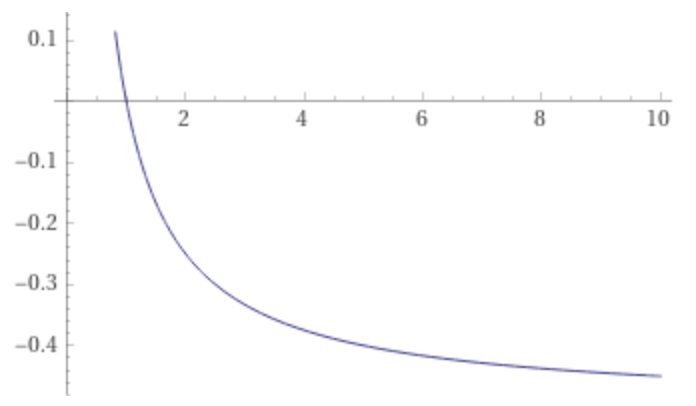
\includegraphics[width=\linewidth]{plot_allocation.png}
  \caption{Allocation with varying alphas}
  \label{fig:llp3}
\end{figure}

\section{CRRA Calculation}
We have:
$$ U(x) = \log(x)$$
And we have:
\begin{align*}
U'(x) &= \frac{1}{x}\\
U''(x) &= \frac{-1}{x^2}\\
R(x) &= \frac{-U''(x)x}{U'(x)} = 1
\end{align*}
Since we have a lognormal distribution of $log(x) \sim N(\mu,\sigma^2)$, $E[U(x)] = E[\log(x)] = \mu$ by definition. Solving for $\log(x_{CE}) = \mu$ yields $x_{CE} = \exp(\mu)$.

Having recovered the setup we turn to the case where we have an allocation of $\pi$ to the Ito process $S_t$ and $(1-\pi)$ to $R_t$ which is a riskless asset or formally the two options are.
\begin{align*}
dS_t &= \mu S_t dt+ \sigma S_t dz_t\\
dR_t &= r R_t dt
\end{align*} 

Applying Ito's Lemma shows that a fixed allocation $\pi$ in fact behaves as $\log(W_t) \sim N(r+\pi(\mu-r) - \frac{\pi^2\sigma^2}{2}, \pi^2\sigma^2)$

From the calculation above we know that for our utility function we are looking to maximise the quantity
$$r+\pi(\mu-r) - \frac{\pi^2\sigma^2}{2}$$
This is a quadratic equation maximised at:
$$\pi^* = \frac{\mu-r}{\sigma^2}$$

\section{Kelly's Criterion}
With initial wealth $W_0$ and initial bet $fW_0$ we have after a single bet two outcomes:
$$ W = \begin{cases}W_0(1+f\alpha)  \text{  with probability $p$}\\W_0(1-f\beta) \text{  with probability $1-p$} \end{cases}$$
or in log space:

$$ \log(W) = \begin{cases}\log(W_0) + \log(1+f\alpha)  \text{  with probability $p$}\\ \log(W_0)+ \log(1-f\beta) \text{  with probability $1-p$} \end{cases}$$

This gives us the expected log wealth after one bet to be:

$$E[\log(W)] = \log(W_0) + p\log(1+f\alpha) + (1-p)\log(1-f\beta) $$

The derivative of this with respect to $f$ and setting to zero yields:
\begin{align*}
\frac{p\alpha}{1+f\alpha} - &\frac{(1-p)\beta}{1-f\beta} = 0\\
\frac{p\alpha}{1+f\alpha} &= \frac{(1-p)\beta}{1-f\beta}\\
p\alpha(1-f\beta) &= (1+f\alpha)(1-p)\beta\\
p\alpha-p\alpha f \beta &= (1-p)\beta +f\alpha(1-p)\beta\\
p\alpha-p\alpha f \beta &= (1-p)\beta +f\alpha(1-p)\beta\\
f(p\alpha \beta+\alpha(1-p)\beta) &= p\alpha - (1-p)\beta\\
f &= \frac{p\alpha - (1-p)\beta}{\alpha \beta}\\
f &= \frac{p}{\beta} - \frac{1-p}{\alpha}
\end{align*} 

Note that the second derivative at this extrema is:
\begin{align*}
-\frac{p\alpha^2}{(1+f\alpha)^2} - &\frac{(1-p)\beta^2}{(1-f\beta)^2}
\end{align*} 
Since $p$ is between 0 and 1, this quantity is necessarily negative (or zero), meaning this is in indeed a maximum. This makes intuitive sence as you should bet more of your wealth with higher chance of success (larger $p$), higher upside \end{document}
